\documentclass[12pt,a4paper]{ctexart}
\usepackage{geometry}
\geometry{left=2.5cm,right=2.5cm,top=2.0cm,bottom=2.5cm}
% \usepackage[english]{babel}
\usepackage{amsmath,amsthm}
\usepackage{amsfonts}
\usepackage[longend,ruled,linesnumbered]{algorithm2e}
\usepackage{fancyhdr}
\usepackage{array}
\usepackage{listings}
\usepackage{color}
\usepackage{graphicx}
\usepackage{minted}
\usepackage{float}
\usepackage[defaultmono]{droidsansmono}

\graphicspath{{pics/}}
\ctexset{today=small}
\definecolor{codebg}{rgb}{0.95,0.95,0.95}

\input{personal_info/info.tex}

\begin{document}
    \begin{titlepage}
        \heiti
        \vspace*{64pt}
        \begin{center}
            \fontsize{48pt}{0} 算法设计与分析\\
            \vspace*{36pt}
            \fontsize{48pt}{0}{实\quad 验\quad 报\quad 告}\\
            \vspace*{48pt}
            \LARGE(2021\~{}2022 学年度\qquad 第 3 学期)\\
            \vspace*{48pt}
        
            \LARGE 实验名称\ \ \underline{\makebox[200pt]{\ExamTitle}}\\
            \LARGE 实验地点\ \ \underline{\makebox[200pt]{\ExamAddr}}\\
            \LARGE 实验日期\ \ \underline{\makebox[200pt]{\today}}\\
            \LARGE 学生姓名\ \ \underline{\makebox[200pt]{\MyName}}\\
            \LARGE 学生学号\ \ \underline{\makebox[200pt]{\MySID}}\\
            \LARGE 指导教师\ \ \underline{\makebox[200pt]{\TeacherName}}\\
            \vspace*{48pt}
            
            \LARGE 东南大学\quad  计软智学院 \quad 制
        \end{center}
    \end{titlepage}

\title{
  {\heiti \textbf{实验四\ 动态规划}
    \footnote{要求:1、分析题请用书面化语言给出详细分析过程。2、实验请统一使用ex0*-学号-姓名的命名格式,latex版本请附上源代码并打包提交。}
    }
}
\date{}

\maketitle

\section*{\bf \color{black}{一、实验目的及意义}}
\noindent
\begin{enumerate}
	\item[(1)]  掌握动态规划算法的基本思想、求解问题的基本步骤;
	\item[(2)]  掌握动态规划算法的时间复杂度;
	\item[(3)]  学会利用动态规划算法解决实际问题。
\end{enumerate}

\vspace{5pt}

\section*{二、实验内容与结果}
\subsection*{题目1:DNA拼接}
\paragraph{题目内容}
\subparagraph{题目描述}
\begin{itemize}
    \item 已知大量同类型的DNA序列被打散成若干基因片段。这些片段可能有所重叠,也可能长度不一。
    \item 基因片段都用区间进行表示,我们甚至可以对这些片段再切割,例如片段$[0, 7]$可以切割成$[0, 1]+[1, 3]+[3, 7]$三部分。
    \item 我们需要将这些片段进行再切割,并将切割后的片段拼接重组成完整的基因序列$([0, T])$。返回所需片段的最小数目,如果无法完成该任务,则返回$-1$ 。
\end{itemize}

\subparagraph{输入格式}
    \begin{itemize}
        \item 第一行输入完整基因序列的长度$T$;
        \item 第二行输入存在的基因片段个数$N$;
        \item 第三行输入N个基因片段的头尾,如$0 2 4 6$表示两个基因片段$[0,2],[4,6]$。
    \end{itemize}
\subparagraph{输出格式}
    \begin{itemize}
        \item 输出拼接重组成序列所需的最小片段数。
    \end{itemize}

\subparagraph{输入输出样例}
如下表
    \begin{figure}[h]
        \centering
        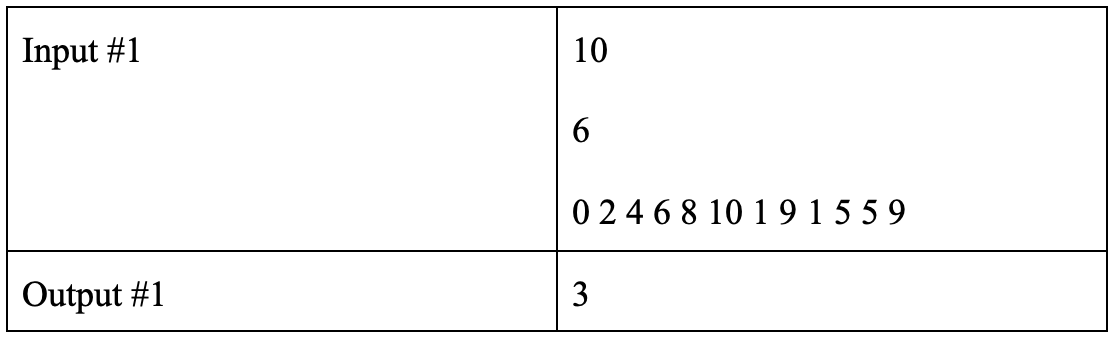
\includegraphics[width=0.80\textwidth]{q1_iodata.png}
    \end{figure}

\vspace{5pt}

\paragraph{实验环境}
\begin{itemize}
    \item 程序设计语言:C++
    \item 编程环境:
    \begin{itemize}
        \item 编辑器:Visual Studio Code (1.67.0)
        \item 编译器:g++ (GCC) 11.2.0
        \item 操作系统:ArchLinux 5.17.5-zen1-1-zen (64-bit)
    \end{itemize}
\end{itemize}

\vspace{5pt}

\paragraph{解答} 时间复杂度:$O(N)$

源码:
\inputminted[bgcolor=codebg,frame=lines,autogobble,linenos=true,breaklines]{cpp}{src/t1.cpp}

\vspace{5pt}

\paragraph{实验结果}
(可附上截图)

\newpage


\subsection*{题目2:股票买卖}
\paragraph{题目内容}
\subparagraph{题目描述}
\begin{itemize}
    \item 给定一个整数数组,其中第 i 个元素代表了第 i 天的股票价格 。设计一个算法计算出最大利润。在满足以下约束条件下,你可以尽可能地完成更多的交易(多次买卖一支股票):
    \item 你不能同时参与多笔交易(你必须在再次购买前出售掉之前的股票)。
    \item 卖出股票后,你无法在第二天买入股票 (即冷冻期为 1 天)。
\end{itemize}

\subparagraph{输入格式}
    \begin{itemize}
        \item 第一行输入股票可交易天数,即数组长度N;
        \item 第二行输入每天的股票价格。
    \end{itemize}

\subparagraph{输出格式}
    \begin{itemize}
        \item 输出最大获利总额。
    \end{itemize}
    
\subparagraph{输入输出样例}
如下表
    \begin{figure}[h]
        \centering
        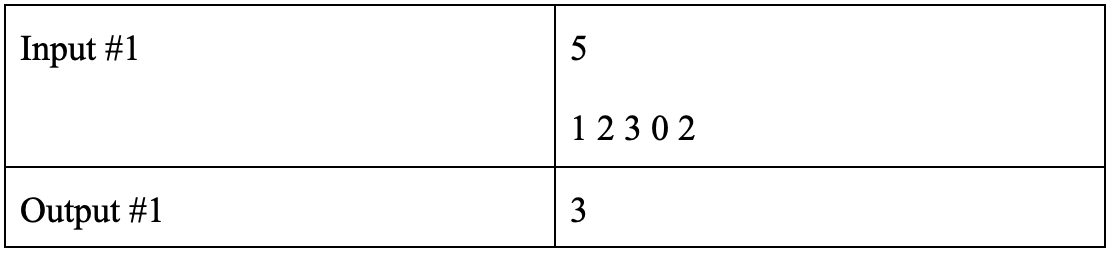
\includegraphics[width=0.80\textwidth]{q2_iodata.png}
    \end{figure}


\vspace{5pt}

\paragraph{实验环境}
\begin{itemize}
    \item 程序设计语言:C++
    \item 编程环境:
    \begin{itemize}
        \item 编辑器:Visual Studio Code (1.67.0)
        \item 编译器:g++ (GCC) 11.2.0
        \item 操作系统:ArchLinux 5.17.5-zen1-1-zen (64-bit)
    \end{itemize}
\end{itemize}

\vspace{5pt}

\paragraph{解答} 时间复杂度:$O(N)$

源码:
\inputminted[bgcolor=codebg,frame=lines,autogobble,linenos=true,breaklines]{cpp}{src/t2.cpp}

\vspace{5pt}

\paragraph{实验结果}
(可附上截图)

\newpage


\subsection*{题目3:自定义编码}
\paragraph{题目内容}
\subparagraph{题目描述}

\begin{itemize}
    \item 给定n个排好序的英文字母(各不相同),按照如下规则创造新的编码表:
    \item 将字符划分为m个集合;
    \item 从每个集合中依次各取一个字符,组成一个m长度的字母;
    \item 重复第2步操作,第k次组成的字母对应编码就是数字k。
    \item 问:通过该方式产生的编码能表示的最大数字是多少?
\end{itemize}

\subparagraph{输入格式}
    \begin{itemize}
        \item 输入编码空间的规模T。
    \end{itemize}

\subparagraph{输出格式}
    \begin{itemize}
        \item 输出编码能表示的最大数字。
    \end{itemize}
    

\subparagraph{输入输出样例}
如下表
    \begin{figure}[h]
        \centering
        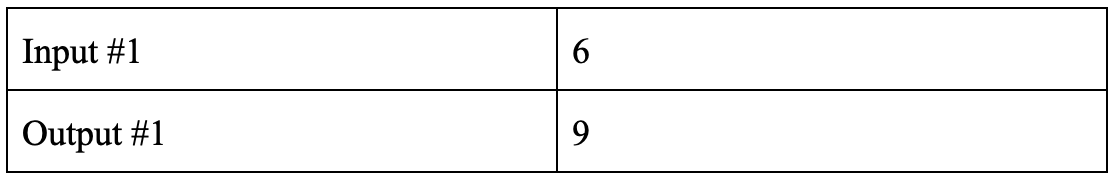
\includegraphics[width=0.80\textwidth]{q3_iodata.png}
    \end{figure}

\vspace{5pt}

\paragraph{实验环境}
\begin{itemize}
    \item 程序设计语言:C++
    \item 编程环境:
    \begin{itemize}
        \item 编辑器:Visual Studio Code (1.67.0)
        \item 编译器:g++ (GCC) 11.2.0
        \item 操作系统:ArchLinux 5.17.5-zen1-1-zen (64-bit)
    \end{itemize}
\end{itemize}

\vspace{5pt}

\paragraph{解答} 时间复杂度:$O(n^3)$

源码:
\inputminted[bgcolor=codebg,frame=lines,autogobble,linenos=true,breaklines]{cpp}{src/t3.cpp}

\vspace{5pt}

\paragraph{实验结果}
(可附上截图)

\newpage

\section*{三、心得体会}
    可根据“实验思考”部分作答,也可以根据个人具体体会作答。自己算法的创新点可在此处进行介绍,酌情加分。

\end{document} 
